\documentclass[10pt]{article}
\usepackage[italian]{babel}
\linespread{1.3}
\usepackage[a4paper, total={6in, 8in}]{geometry}
\usepackage{graphicx,hyperref,wrapfig,ragged2e}
\hypersetup{
    colorlinks=true,
    linkcolor=cyan,
    filecolor=magenta,
    urlcolor=cyan,
    pdftitle={Relazione Marangon Matteo}
}
\justifying

\title{Relazione progetto - Programmazione ad Oggetti}
\author{Marangon Matteo - matricola n$^{\circ}$ 2009094}
\date{A.A. 2024/2025}

\begin{document}

\begin{figure}
    \centering
    
\includegraphics[width=0.3\textwidth]{./unipdlogo.png}
\end{figure}
\maketitle

\newpage

\begin{figure} [h]
    \centering
    
\includegraphics[width=0.1\textwidth]{./vaporlogo.png}
\end{figure}
\section{Introduzione} % circa 200 parole, no immagini !
Vapor è un software che permette di visualizzare la propria libreria digitale di software, videogiochi, DLC e colonne sonore. Si possono aggiungere, modificare, cercare e rimuovere gli elementi della libreria, ciascuno con dei propri attributi caratteristici e una differente visualizzazione grafica. È anche possibile importare una propria libreria in formato JSON, modificarla a piacimento e salvarla per un utilizzo continuo nel tempo, oltre a godere di una serie di funzionalità aggiuntive elencate nel capitolo \ref{funzionalita}.
\\Ho scelto questo argomento per interesse personale nel mondo dei videogiochi e, nello specifico, perché ho sempre prestato attenzione a come vengono sviluppati i launcher (Steam, Epic Games, Ubisoft, EA, ecc.) e quali scelte vengono adottate da ciascun produttore nel corso degli anni. Questi esempi sono stati fonte di ispirazione per le categorie, gli attributi e alcuni elementi di presentazione estetica, benché il progetto sia estremamente ridotto in confronto.
\\Il progetto è stato testato su un dispositivo personale con sistema operativo Windows 11 e sulla macchina virtuale fornita con Linux, distribuzione Ubuntu 22.04.

\section{Descrizione del modello}
Il modello logico di Vapor si articola in una gerarchia di classi che rappresentano i diversi tipi di oggetti e le loro caratteristiche. In cima a questa gerarchia si trova la classe astratta AbstractItem, che definisce le proprietà comuni a tutti i media: id, nome, descrizione e percorso dell'immagine. Questa classe è la base per la costruzione di classi concrete che rappresentano specifici tipi di elementi della libreria, ovvero Software, Videogame, DLC e Soundtrack. Si noti che l'attributo id di AbstractItem, che viene poi ereditato dalle classi derivate, non viene mai usato o modificato attivamente dall'utente, bensì viene utilizzato unicamente per distinguere in maniera univoca gli elementi della libreria per interazioni come la cancellazione, la modifica o l'ordinamento.
\begin{figure} [h] \label{fig:uml}
    \centering
    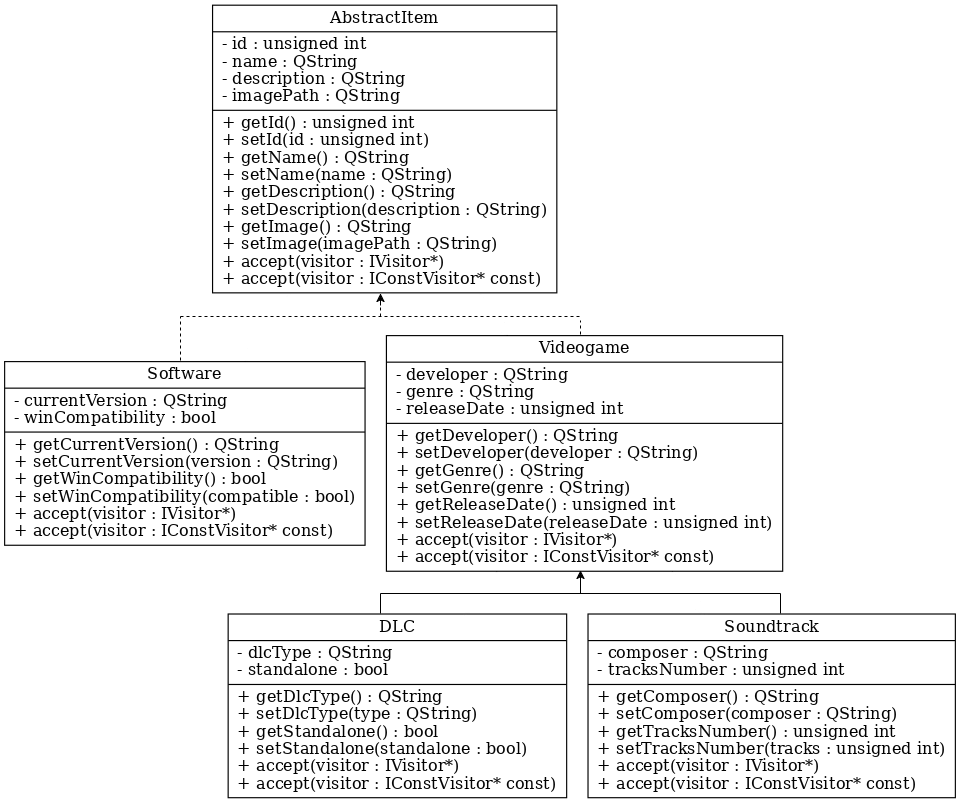
\includegraphics[width=0.9\textwidth]{./uml_diagram.png}
    \caption{Diagramma UML delle principali classi del modello}
\end{figure}
Il diagramma UML \hyperref[fig:uml]{qui} presente fornisce un'idea della struttura piuttosto tradizionale adottata per Vapor.
La scelta di utilizzare una classe AbstractItem come classe di base astratta non presenta particolari peculiarità, e ciascuna classe ha dei classici metodi setter e getter che adempiono al loro scopo. Le classi DLC e Soundtrack, invece, sono state derivate direttamente da Videogame poiché si presuppone che esse abbiano sempre un videogioco base di cui fanno parte: anche se quest'ultimo non dovesse risiedere all'interno della stessa libreria, verranno ereditati gli attributi (genere, sviluppatore, data di rilascio) che permetteranno di rendere evidente il videogioco di appartenenza. Nel diagramma si accenna anche a metodi accept destinati all'utilizzo dei visitor; sono state definite le interfacce IVisitor e IConstVisitor che consentono di estendere le funzionalità delle classi AbstractItem senza modificarle.
\\La separazione tra modello e vista è un aspetto fondamentale del design dell'applicazione: il codice del modello è riutilizzabile e indipendente dall'interfaccia utente, garantendo una maggiore flessibilità e manutenibilità.

\newpage
\section{Polimorfismo}
L'uso del polimorfismo è fondamentale per la gestione dei diversi tipi di media, ed è implementato attraverso le interfacce IVisitor e IConstVisitor.
\\Un esempio di polimorfismo non banale si trova proprio in questo Visitor pattern: le classi ItemRenderer, SetItemVisitor, EditItemVisitor e SearchItemVisitor implementano l'interfaccia IConstVisitor o IVisitor per eseguire operazioni diverse su ciascun tipo di oggetto.
\begin{itemize}
    \item \textbf{ItemRenderer}: utilizza il polimorfismo per visualizzare correttamente ogni tipo di media, creando widget personalizzati in base al tipo dinamico dell'oggetto: i videogiochi saranno visualizzati con una copertina verticale, i DLC avranno in sovrimpressione una freccia di download, le soundtrack saranno renderizzate con l'immagine di un disco e i software con una copertina orizzontale. La classe inoltre implementa il pattern Visitor anche per gestire le diverse visualizzazioni a griglia, lista e dettagli in base al tipo di media che deve renderizzare;
    \item \textbf{SetItemVisitor}: è utilizzato per prelevare i dati dagli attributi degli oggetti e inserirli nella vista dedicata alla modifica degli oggetti;
    \item \textbf{EditItemVisitor}: è utilizzato per applicare le modifiche apportate dagli utenti ai vari attributi degli oggetti;
    \item \textbf{SearchItemVisitor}: è dedicato alla ricerca per filtrare e cercare oggetti sulla base di una stringa e un filtro per tipo;
    \item \textbf{JsonVisitor}: è utilizzato per l'implementazione della persistenza dei dati su file JSON, illustrata nel dettaglio nel capitolo \ref{persistenza}.
\end{itemize}
Questi visitor dimostrano come il polimorfismo permette di eseguire operazioni diverse in base al tipo di oggetto, evitando controlli espliciti sul tipo. Un altro esempio minore di polimorfismo si trova nella gestione delle immagini: la classe AbstractItem include un metodo setImage che controlla se l'immagine esiste e, in caso contrario, assegna un'immagine di default diversa a seconda del tipo di media tramite DefaultImageVisitor.

\section{Persistenza dei dati} \label{persistenza}
La persistenza dei dati in Vapor è gestita tramite file JSON, formato scelto per la sua leggibilità e facilità di manipolazione. La classe JsonItemSaver serializza gli oggetti del modello in formato JSON, mentre la classe JsonItemLoader deserializza i dati dal file, creando gli oggetti corrispondenti da visualizzare nel software. Questo file contiene un array di oggetti ciascuno rappresentante un elemento, come ci si aspetterrebbe da un comune file JSON. Il processo di salvataggio prevede la creazione di un file con questa struttura, mentre il caricamento dei dati segue il processo inverso: viene letto il file JSON scelto da finestra di dialogo di sistema, vengono creati gli oggetti corrispondenti e popolata la collezione di media.
\\Un esempio di una ricca libreria per Vapor è fornito con il codice del progetto (nel file \textit{data/library.json}) che viene aperto automaticamente all'avvio del software.

\section{Funzionalità implementate} \label{funzionalita}
Vapor offre una serie di funzionalità oltre a quelle richieste dalle specifiche, sia strutturali che estetiche:
\\Funzionalità principali:
\begin{itemize}
    \item Gestione di quattro tipi di media: ognuno di essi ha attributi specifici e una visualizzazione personalizzata;
    \item Ricerca in tempo reale e filtro: l'applicazione permette di cercare per nome, descrizione, sviluppatore, compositore o genere, e di filtrare per tipo di oggetto;
    \item Ordinamento: gli elementi possono essere ordinati per nome, id e per tipo.
\end{itemize}
Funzionalità estetiche e di usabilità:
\begin{itemize}
    \item Visualizzazione in diverse modalità: sono implementate visualizzazioni a griglia, in lista o in dettaglio, oltre a quelle dedicate all'aggiunta e alla modifica di elementi;
    \item Menu e toolbar: l'applicazione offre un menu per le operazioni di file e gestione dei media, oltre a una toolbar spostabile con funzioni di ricerca e ordinamento;
    \item Status bar: vengono visualizzati messaggi di stato per tenere informato l'utente sull'operazione appena eseguita;
    \item Stili e temi: l'interfaccia utente utilizza un foglio di stile (\textit{style.qss}) per garantire un aspetto coerente;
    \item Icone: sono utilizzate icone per rendere più intuitive le operazioni disponibili;
    \item Effetti grafici: sono presenti effetti grafici come il cambio di colore al passaggio del mouse per migliorare l'interazione;
    \item Immagini predefinite: sono utilizzate immagini predefinite per i vari tipi di oggetti nel caso in cui non venga selezionata un'immagine dall'utente.
\end{itemize}

\newpage
\section{Rendiconto ore}
Il monte ore è stato superato rispetto a quanto preventivamente stimato in quasi tutte le attività. Lo studio del framework Qt mi ha messo in difficoltà ed impararne tutte le peculiarità è stato certamente una sfida; questo mi ha portato ad oltrepassare le ore previste anche in quanto a scrittura del codice nel mio personale percorso di apprendimento. Inoltre, alcune difficoltà nel trovare l'origine di problemi nati durante lo sviluppo del software hanno fatto crescere anche il numero di ore di debug. Le ore dedicate allo sviluppo meramente estetico, alla ricerca delle immagini, delle icone e dell'arricchimento della libreria naturalmente non sono state conteggiate.
\begin{center}
    \begin{tabular}{| c | c | c |} \hline
    Attività & Ore previste & Ore effettive \\\hline
    Studio e progettazione & 5 & 6 \\
    Studio del framework Qt & 6 & 9 \\
    Sviluppo del codice del modello & 10 & 16 \\
    Sviluppo del codice della GUI & 10 & 18 \\
    Test e debug & 5 & 11 \\
    Stesura della relazione & 4 & 4 \\\hline
    Totale & 40 & 64 \\\hline
    \end{tabular}
\end{center}

\end{document}
